% DOC SETTINGS ===================================
\documentclass{article}
\usepackage[utf8]{inputenc}
\usepackage{steinmetz}
\usepackage{mathtools}  
\usepackage{multicol}
\usepackage{circuitikz}
\usepackage{tikz}
\usepackage{listings}
\usepackage{geometry}
\usepackage{fancyhdr}
\usepackage{graphicx}
\usepackage{lmodern}
\usepackage{amsfonts}
\usepackage{media9}
\usepackage{parskip}
\usetikzlibrary{positioning, fit, calc}
\pagestyle{fancy}
\lhead{ECE2714 Problem Set 10}
\rhead{Kavin Thirukonda 2021}
\fancyheadoffset{0mm}
 \geometry{
 a4paper,
 total={170mm,257mm},
 left=20mm,
 top=25mm,
 }
\mathtoolsset{showonlyrefs} 
\cfoot{}
% DOC SETTINGS ===================================
\begin{document}
\begin{enumerate}
    \item Consider the second-order "Sallen-Key" filter below
    \begin{center}
    \begin{circuitikz} [american voltages]
    \draw (0,0) node[op amp](amp){};
    \draw (amp.-) to [short] ($(amp.-)+(-1.5,0)$)
    to [C, l=$C_2$] ($(amp.-)+(-1.5,-2.5)$)
    to [short,-o] ($(amp.-)+(3.5,-2.5)$); 
    \draw (amp.out) to [short,-o] ($(amp.out)+(1.15,0)$)
    to [open, v=$y(t)$] ($(amp.-)+(3.5,-2.5)$);
    \draw (amp.+) to [short] ($(0,-.75)+(amp.+)$)
    to [short]($(2.38,-.75)+(amp.+)$)
    to [short](amp.out);
    \draw (amp.out) to [short] ($(0,1.5)+(amp.out)$)
    to [C, l =$C_1$] ($(-6,1.5)+(amp.out)$)
    to [short] ($(-6,.5)+(amp.out)$)
    to [R,l=$R_2$]($(amp.-)+(-1.5,0)$);
    \draw ($(-6,.5)+(amp.out)$) to [R, l_=$R_1$,-o] ($(-8,.5)+(amp.out)$)
    to [open, v=$x(t)$] ($(-8,-2)+(amp.out)$)
    to [short,o-] ($(amp.-)+(-1.5,-2.5)$);
    \end{circuitikz} 
    \end{center}
    which is described by the following frequency response
    \begin{equation}
        H(j\omega) = \frac{\omega_o^2}{\omega_o^2-\omega^2+j2\alpha\omega}
    \end{equation}
    where
    \begin{equation}
        \alpha = \frac{R_1 + R_2}{2R_1R_2C_1}\text{ and }\omega_o^2 = \frac{1}{R_1R_2C_1C_2}
    \end{equation}
    \begin{enumerate}
        \item Let $R_1 = 12k\Omega, R_2 = 200k\Omega, C_1 = 1nF, C_2 = 100pF.$ Plot the frequency response as a bode plot using Matlab from 1Hz to 30kHz
        \begin{center}
            \boxed{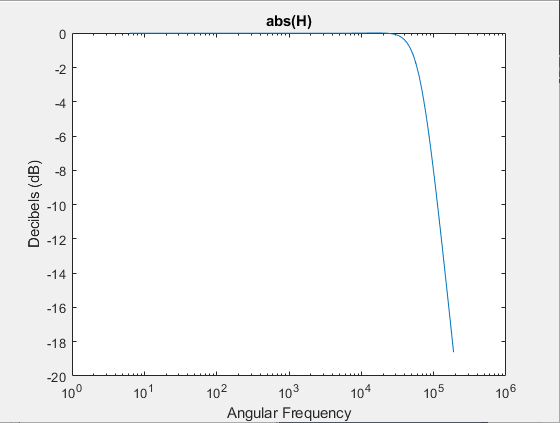
\includegraphics[width = .4\textwidth]{matlabmag.png}}
            \boxed{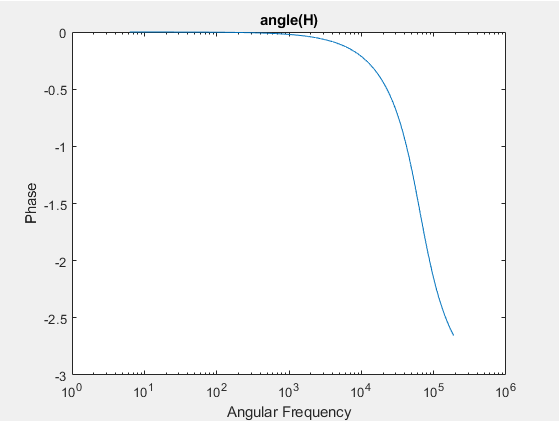
\includegraphics[width = .4\textwidth]{matlabangle.png}}
        \end{center}
        \item Determine the output when the input is
        \begin{equation}
            x(t) = \cos(2\pi\cdot5000t) + \cos(2\pi\cdot10000t)+\cos(2\pi\cdot20000t)
        \end{equation}
        \begin{center}
            The output would be:
        \end{center}
        \begin{equation}
            y(t) = -.1\cos(2\pi\cdot5000t- 0.7185) + -2.50\cos(2\pi\cdot10000t  - 1.5)+ -11.75\cos(2\pi\cdot20000t - 2.4)
        \end{equation}
    \end{enumerate}
    \newpage
    \item Simulate the cirucit in Problem 1a in LTSpice, using an ideal op-amp model. Perform the following analyses:
    \begin{itemize}
        \item Transient analysis (.tran spice directive) of the output for unit amplitude sinusoidal voltage inputs at 5, 10, and 20 kHz.  You should adjust the start and stop times of the transient simulation to show 2-3 steady-state cycles in each case.  Attach the plots.
        \begin{center}
            \textbf{5kHz Transient}
        \end{center}
        \boxed{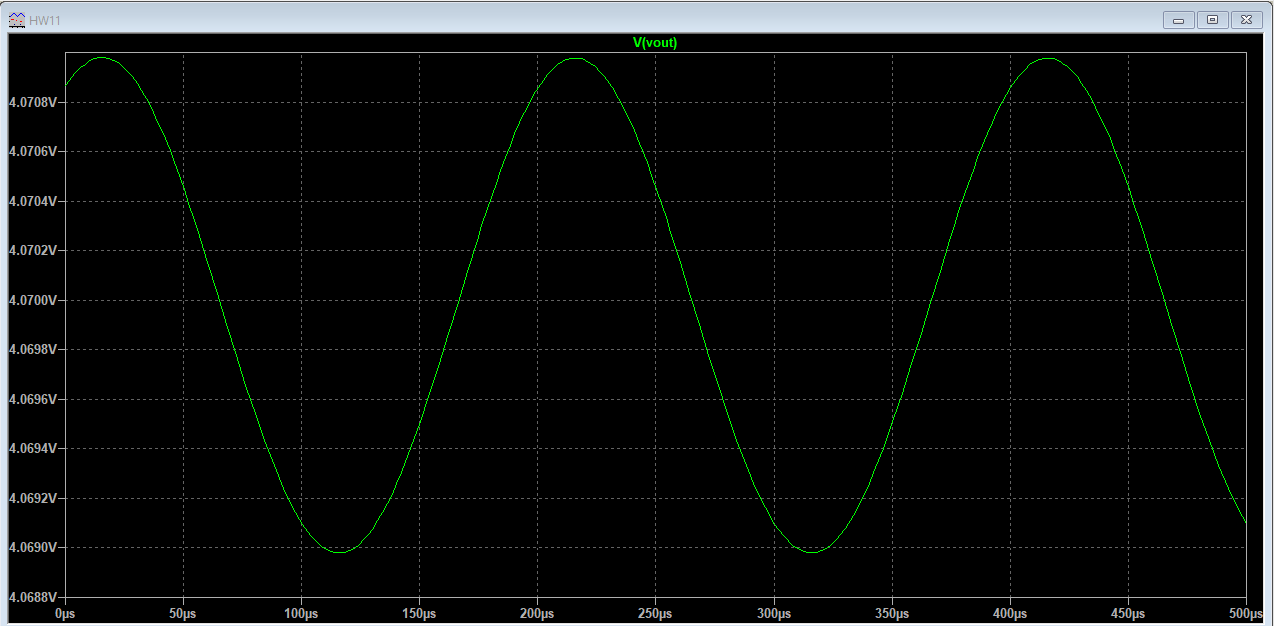
\includegraphics[width = .8\textwidth]{tran1.png}}
        \begin{center}
            \textbf{10kHz Transient}
        \end{center}
        \boxed{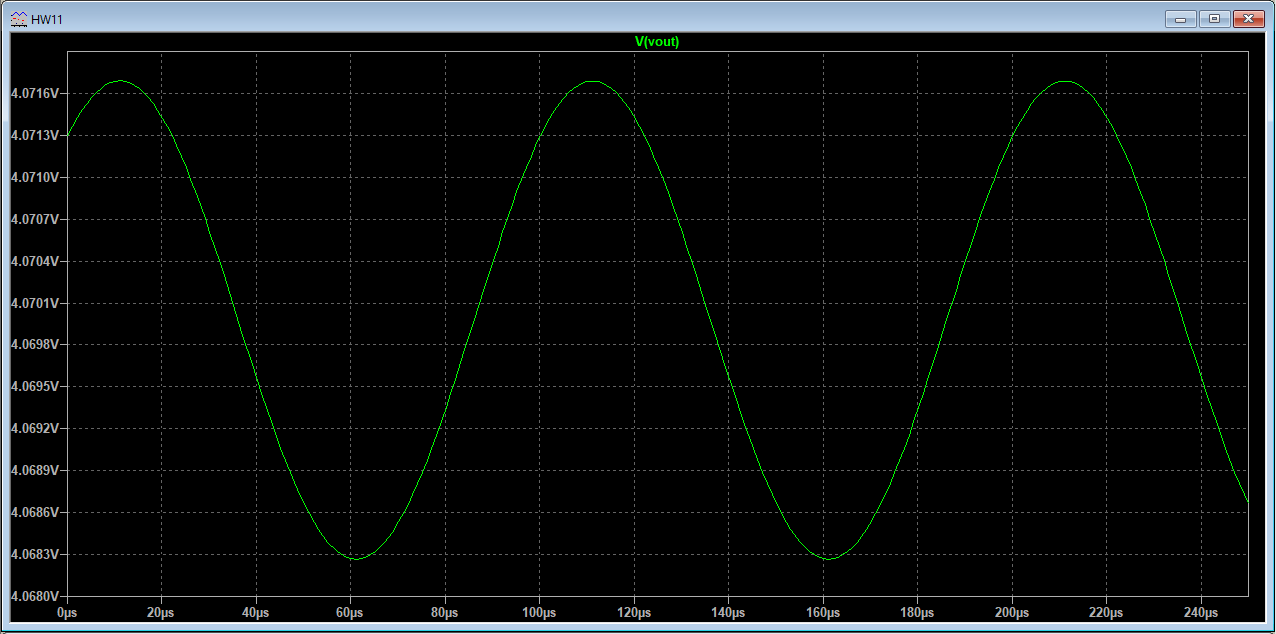
\includegraphics[width = .8\textwidth]{tran2.png}}
        \begin{center}
            \textbf{20kHz Transient}
        \end{center}
        \boxed{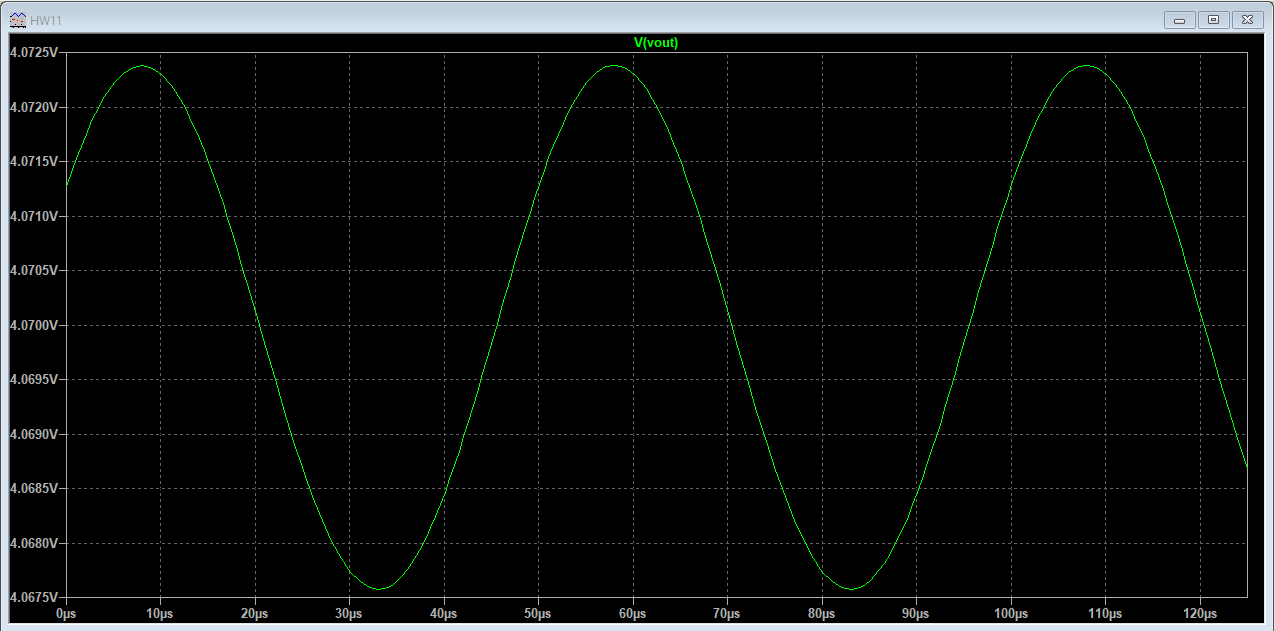
\includegraphics[width = .8\textwidth]{tran3.png}}
        \item Perform a frequency sweep (.ac spice directive) from 1Hz to 30 kHz. Attach the resulting plot.
        \boxed{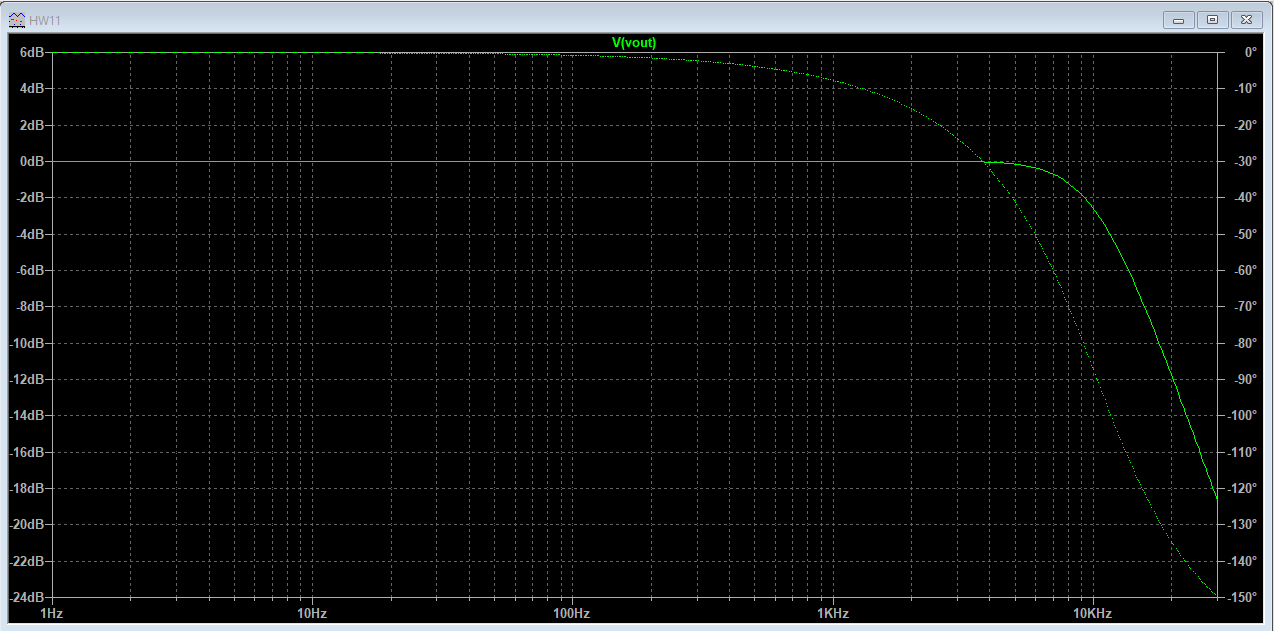
\includegraphics[width = .85\textwidth]{ltbode.png}}
    \end{itemize}
    \begin{enumerate}
        \item From the transient plots estimate the gain and phase shifts between each input-output case. Compare the results to your result in problem 1b.
        \begin{center}
            Some rough estimates are
            
            \textbf{5kHz:}
            
            gain(dB):-.1 phase: -0.7185
            
            \textbf{10kHz:} 
            
            gain(dB):-2.50 phase: -1.5
            
            \textbf{20kHz:} 
            
            gain(dB):-11.75 phase: -2.4
        \end{center}
        \item Compare the frequency sweep simulation to your result in Problem 1a Identify the stop-band and pass-band frequencies in both.
        \begin{center}
            They are quite similar filters, they both have passbands of 0 to around 10kHz.
        \end{center}
    \end{enumerate}
    \newpage
    \item Consider the second-order DT filter given by the difference equation
    \begin{equation}
        a_1y[n+2]+a_2y[n+1]+a_3y[n] = b_1x[n+2]+b_2x[n+1]+b_3x[n]
    \end{equation}
    where $a_1 = 1, a_2 = -0.6071, a_3 = 0.9647, b_1 = 0.9824, b_2 = -0.6071, b_3 = 0.9824.$ Plot the frequency response from $-\pi\text{ to }\pi$. Characterize the type of filter and its relevant parameters.
    \begin{center}
        \boxed{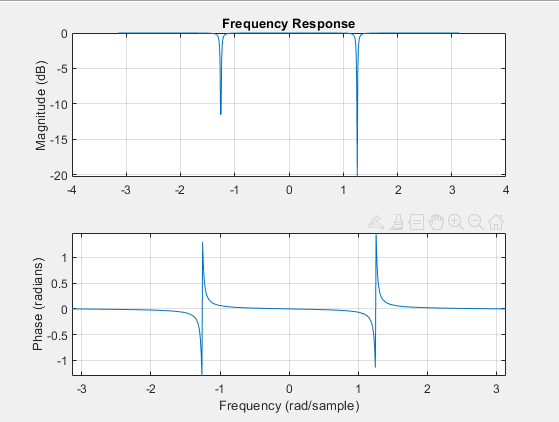
\includegraphics[width = .7\textwidth]{threegraph.png}}
    \end{center}
    \item Read the finite-length DT signal in the file \texttt{corrupted.wav} into Matlab using the \texttt{audioread} command. Compute the discrete fourier transform of the signal using the \texttt{fft} command, and plot the Magnitude (in dB) and phase (in radians per second) for frequencies from 0 to $\pi$.
    \begin{center}
        \boxed{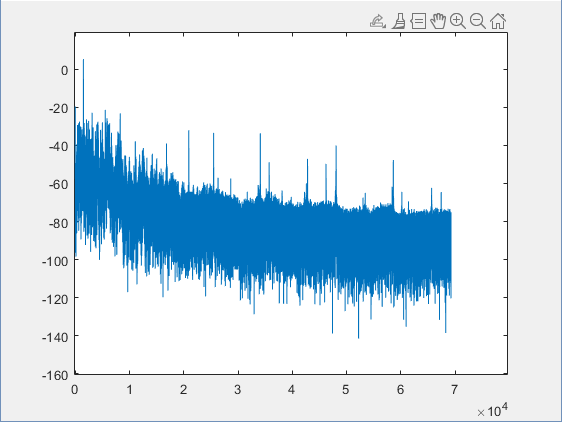
\includegraphics[width = .45\textwidth]{4mag.png}}
        \boxed{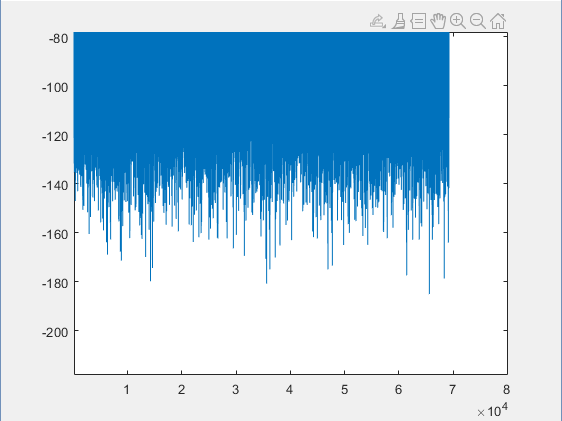
\includegraphics[width = .45\textwidth]{4phase.png}}
    \end{center}
\end{enumerate}
\end{document}
